% !TeX encoding=utf8
% !TeX spellcheck = en-US

\chapter{Publications}
%\markboth{Publications}{Publications}

The following publications of mine formed the basis of this thesis.

%% In these lists the publications are numbered by date of publications
%% and the author of the thesis can be printed in bold.


% \section*{Wissenschaftliche Veröffentlichungen}
\begin{refsection}
\nocite{Halchenko2021, wagner2020datalad, wagner2022fairly}
% NISO2022119623, HankePestilliWagnerMarkiewiczPolineHalchenko+2021+17+25,
\begin{refcontext}[sorting=nyt]  
	\printbibliography[heading=none, resetnumbers=true]
\end{refcontext}
%\end{refsection}

My contributions to these works are as follows:


1) Wagner A.S, Waite L.K., Meyer, K., Heckner, M.K., Kadelka, T., Reuter, N., Waite, A.Q.,  Poldrack, B., Markiewicz, C.J.,  Halchenko, Y.O., Vavra, P., Chormai, P., Poline, J-B., Paas, L-K., Herholz, P., Mochalski, L.N., Kraljevic, N., Wiersch, L., Hutton, A. \& Hanke, M. (2020). The DataLad Handbook. Zenodo, 10. \url{https://doi.org/10.5281/zenodo.3608611}.\\
\forceindent I conceived the conceptual structure and educational concept, co-created the technical backbone, coordinated development efforts and community management, and wrote most of its contents.
I have also further refined the contents and its layout, and published it as a physical book (ISBN: 979-8-85-703797-3).

2) Halchenko, Y.O., Meyer, K., Poldrack, B., Solanky, S., Wagner, A.S, Gors, J., MacFarlane, D., Pustina, D., Sochat, V., Gosh, S.S., Mönch, C., Markiewicz, C.J., Waite, L.K., Shlyakhter, I., de la Vega, A., Hayashi, S., Häusler, C.O., Poline, J-B., Kadelka, T., Skyten, K., Jareka, D., Kennedy, D., Strauss, T., Cieslak, M., Ioanas, H.I., Vavra, P., Schneider, R., Pflüger, M., Haxby, J.V., Eickhoff, S.B., \& Hanke, M. (2021). DataLad: Distributed system for joint management of code, data, and their relationship. Journal of Open Source Software, 6(63). 3262. \url{https://doi.org/10.21105/joss.03262} \\
\forceindent I contributed to the conceptualization, writing, and editing of the manuscript, and have been a regular contributor to the underlying software since 2019. With the exception of the first and last author, the order of authors was determined by the amount of committed code contributions.

3) Wagner, A.S., Waite, L.K., Wierzba, M., Hoffstaedter, F., Waite, A.Q., Poldrack, B., Eickhoff, S.B. \& Hanke, M. (2022). Fairly big: A framework for computationally reproducible processing of large-scale data. Scientific data, 9(1), 80\\
\forceindent I co-conceived the setup of the framework, co-piloted and documented an earlier version of the framework with a smaller dataset, co-implemented the open workflow, wrote the first draft of the manuscript, and contributed to the conceptualization, writing, and editing of the manuscript.

The original publications from \citet{Halchenko2021} and \citet{wagner2022fairly} are included hereafter.

% \section*{Beiträge auf internationalen Konferenzen}
%\begin{refsection}
%\nocite{wagner202310, wagnerohbm2022, wagnerohbm2021, poldrackohbm2020, wagner_adina_s_2020_7906718}

%\printbibliography[env=numbered+bold, heading=none, sorting=ynt, resetnumbers=true]
%\begin{refcontext}[sorting=nyt]
%	\printbibliography[heading=none, resetnumbers=true]
%\end{refcontext}
%\end{refsection}

% \section*{Beiträge auf nationalen Konferenzen}
%\begin{refsection}
%\nocite{adina_s_wagner_2021_4541323}

%\printbibliography[env=numbered+bold, heading=none, sorting=ynt, resetnumbers=true]
%\begin{refcontext}[sorting=nyt]
%	\printbibliography[heading=none, resetnumbers=true]
%\end{refcontext}


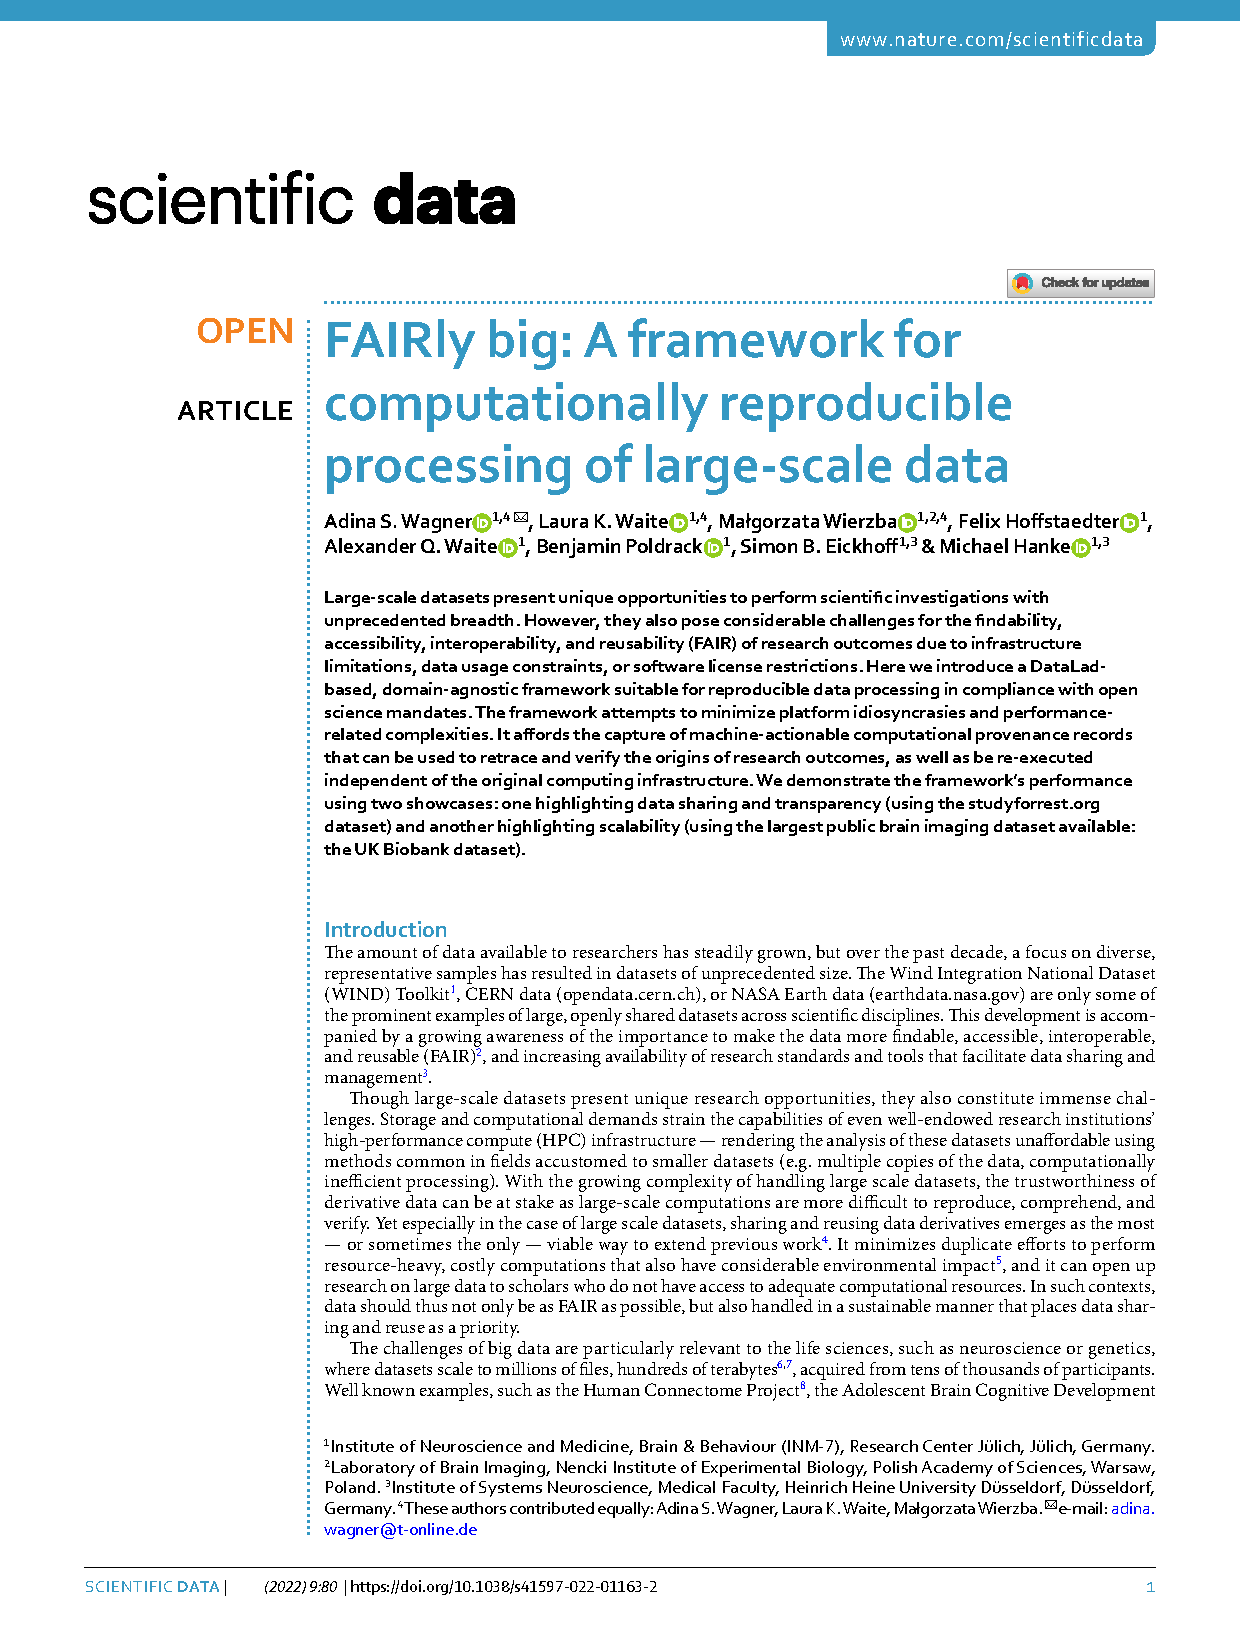
\includepdf[pages=1-17]{content/appendix_pub_fairlybig.pdf}
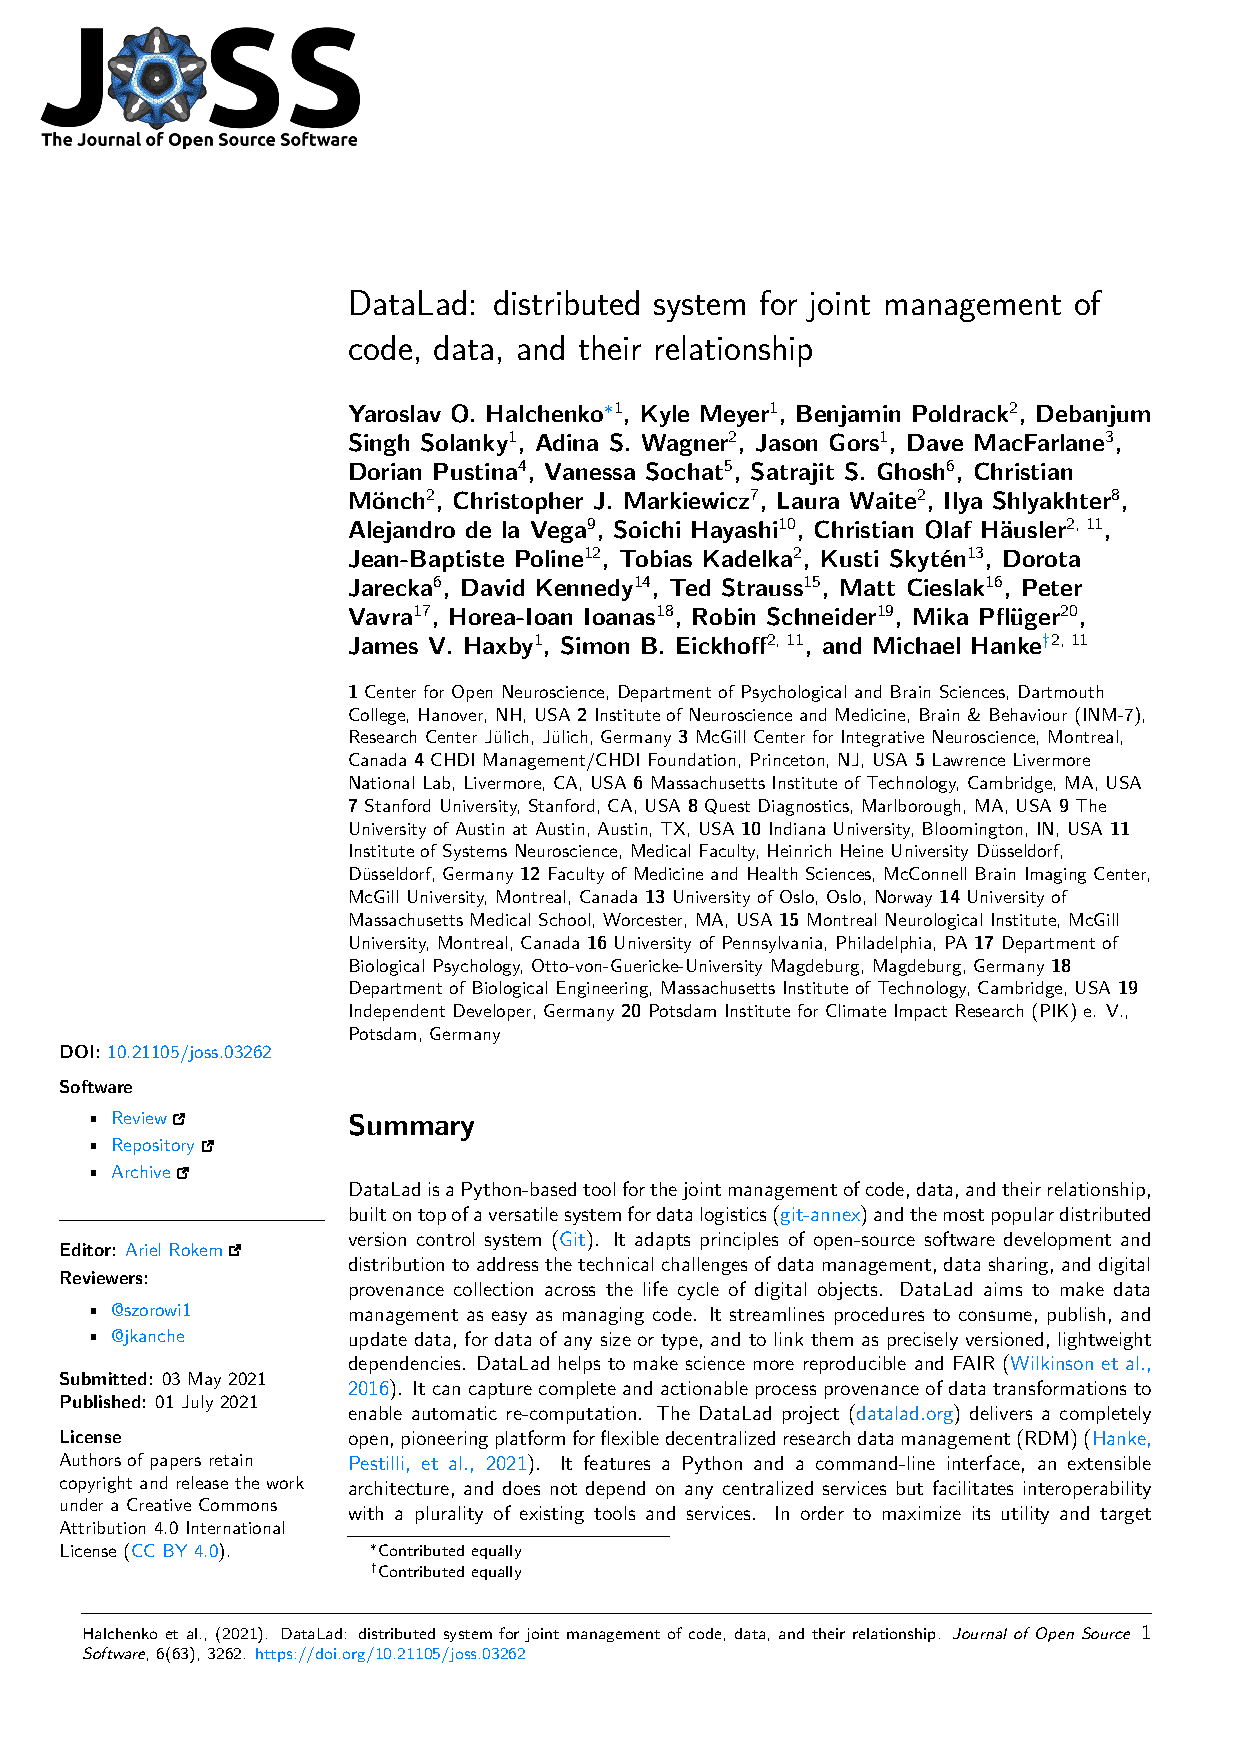
\includepdf[pages=1-8]{content/appendix_pub_datalad.pdf}

\end{refsection}
%
